
\documentclass{report}
\usepackage{amssymb, amsmath}
\usepackage{graphicx}
\usepackage{float}

\title{Reporte Tarea 5}
\date{14 de Noviembre de 2022}
\author{Nestor Adrian Sandoval Ortiz}

\begin{document}
    \maketitle

    \chapter{Problema 1}

    \begin{tabular}{l|c|c|c|c|c|c}
        Instancia & \multicolumn{2}{|c|}{Mejor solucion} & \multicolumn{2}{|c|}{Peor solucion} & \multicolumn{2}{|c|}{Solucion promedio}\\
        \hline
        & Valor & Peso & Valor & Peso & Valor & Peso\\
        \hline
        ks-4-0 & 19 & 11 & 12.0 & 7.0 & 18.04 & 9.96\\
        \hline
        ks-19-0 & 12248 & 30996 & 8142.0 & 21384.0 & 10919.44 & 28126.88\\
        \hline
        ks-30-0 & 99764 & 99779 & 89750.0 & 89751.0 & 98822.04 & 98830.08\\
        \hline
        ks-40-0 & 99913 & 99896 & 96003.0 & 96001.0 & 99209.0 & 99197.9\\
        \hline
        ks-45-0 & 23974 & 58148 & 14564.0 & 35728.0 & 19199.88 & 46885.76\\
        \hline
        ks-50-0 & 141611 & 341022 & 130467.0 & 314634.0 & 138971.06 & 335644.12\\
        \hline
        ks-50-1 & 5210 & 4988 & 4694.0 & 4795.0 & 4943.64 & 4884.46\\
        \hline
        ks-60-0 & 99779 & 99809 & 87750.0 & 87751.0 & 98323.66 & 98338.32\\
        \hline
        ks-82-0 & 104710920 & 104710920 & 9.4529142e7 & 9.4529142e7 & 1.02801462e8 & 1.02801462e8\\
        \hline
        ks-100-0 & 99796 & 99843 & 93766.0 & 93783.0 & 98747.52 & 98771.04\\
        \hline
        ks-100-1 & 1331419 & 3187738 & 1.127287e6 & 2.699574e6 & 1.28013444e6 & 3.06689488e6\\
        \hline
        ks-100-2 & 10473 & 9873 & 9395.0 & 9258.0 & 9895.8 & 9768.28\\
        \hline
        ks-106-0 & 106917397 & 106917397 & 8.5361792e7 & 8.5361792e7 & 1.0100383372e8 & 1.0100383372e8\\
        \hline
        ks-200-0 & 99935 & 99842 & 79501.0 & 79500.0 & 90265.12 & 90249.56\\
        \hline
        ks-200-1 & 1095937 & 2637974 & 1.06421e6 & 2.57162e6 & 1.08485316e6 & 2.61725032e6\\
        \hline
        ks-300-0 & 1680290 & 4036980 & 1.620773e6 & 3.904646e6 & 1.67077534e6 & 4.02019468e6\\
        \hline
        ks-400-0 & 3955280 & 9485160 & 3.794975e6 & 9.10725e6 & 3.9228375e6 & 9.411907e6\\
        \hline
        ks-500-0 & 52317 & 49903 & 45654.0 & 46136.0 & 49955.48 & 49008.28\\
        \hline
        ks-1000-0 & 104559 & 98890 & 92272.0 & 94357.0 & 98633.84 & 97372.88\\
        \hline
        ks-10000-0 & 1037704 & 999890 & 944474.0 & 964875.0 & 994545.5 & 982512.58               
        
    \end{tabular}

    \chapter{Problema 2}

    \begin{tabular}{l|c|c|c}
        Instancia & Mejor Solucion & Solucion Promedio & Peor Solucion\\
        \hline
        & Suma de Distancias & Suma de Distancias & Suma de Distancias\\
        \hline
        kcenter-1 & 34187.2 & 35943.13999999999 & 38943.3\\
        \hline
        kcenter-2 & 1310.75 & 1605.8989999999994 & 1918.82\\
        \hline
        kcenter-3 & 1900.48 & 2019.1342000000006 & 2228.0\\
        \hline
        kcenter-4 & 3785.08 & 3989.5181999999995 & 4401.32\\
        \hline
        kcenter-5 & 2926.1 & 3048.157200000001 & 3254.96\\
        \hline
        kcenter-6 & 6849.27 & 7212.512199999998 & 7725.54\\
        \hline
        kcenter-7 & 8.11192e7 & 8.126886e7 & 8.52988e7\\
        \hline
        kcenter-8 & 1.99967e8 & 2.0821136e8 & 2.22676e8\\
            
    \end{tabular}
    \pagebreak

    \section{kcenter-1}
        \begin{figure}[H]
            \includegraphics[width=\linewidth]{/Users/lloydna/Desktop/UP/5° Semestre/Optimizacion/Optimizacion/Tareas/Tarea5/Parte2/Codigos/kcenter-1/GraficaCenters.png}
            \caption{Mejores centros encontrados}
            \label{fig:kc11}
        \end{figure}

        \begin{figure}[H]
            \includegraphics[width=\linewidth]{/Users/lloydna/Desktop/UP/5° Semestre/Optimizacion/Optimizacion/Tareas/Tarea5/Parte2/Codigos/kcenter-1/GraficaColors.png}
            \caption{Distribucion de puntos por centro}
            \label{fig:kc12}
        \end{figure}

        \begin{figure}[H]
            \includegraphics[width=\linewidth]{/Users/lloydna/Desktop/UP/5° Semestre/Optimizacion/Optimizacion/Tareas/Tarea5/Parte2/Codigos/kcenter-1/GraficaTiny.png}
            \caption{Distribucion de puntos por centro (miniatura)}
            \label{fig:kc13}
        \end{figure}

    \pagebreak

    \section{kcenter-2}
        \begin{figure}[H]
            \includegraphics[width=\linewidth]{/Users/lloydna/Desktop/UP/5° Semestre/Optimizacion/Optimizacion/Tareas/Tarea5/Parte2/Codigos/kcenter-2/GraficaCenters.png}
            \caption{Mejores centros encontrados}
            \label{fig:kc21}
        \end{figure}

        \begin{figure}[H]
            \includegraphics[width=\linewidth]{/Users/lloydna/Desktop/UP/5° Semestre/Optimizacion/Optimizacion/Tareas/Tarea5/Parte2/Codigos/kcenter-2/GraficaColors.png}
            \caption{Distribucion de puntos por centro}
            \label{fig:kc22}
        \end{figure}

        \begin{figure}[H]
            \includegraphics[width=\linewidth]{/Users/lloydna/Desktop/UP/5° Semestre/Optimizacion/Optimizacion/Tareas/Tarea5/Parte2/Codigos/kcenter-2/GraficaTiny.png}
            \caption{Distribucion de puntos por centro (miniatura)}
            \label{fig:kc23}
        \end{figure}

    \pagebreak

    \section{kcenter-3}
        \begin{figure}[H]
            \includegraphics[width=\linewidth]{/Users/lloydna/Desktop/UP/5° Semestre/Optimizacion/Optimizacion/Tareas/Tarea5/Parte2/Codigos/kcenter-3/GraficaCenters.png}
            \caption{Mejores centros encontrados}
            \label{fig:kc31}
        \end{figure}

        \begin{figure}[H]
            \includegraphics[width=\linewidth]{/Users/lloydna/Desktop/UP/5° Semestre/Optimizacion/Optimizacion/Tareas/Tarea5/Parte2/Codigos/kcenter-3/GraficaColors.png}
            \caption{Distribucion de puntos por centro}
            \label{fig:kc32}
        \end{figure}

        \begin{figure}[H]
            \includegraphics[width=\linewidth]{/Users/lloydna/Desktop/UP/5° Semestre/Optimizacion/Optimizacion/Tareas/Tarea5/Parte2/Codigos/kcenter-3/GraficaTiny.png}
            \caption{Distribucion de puntos por centro (miniatura)}
            \label{fig:kc33}
        \end{figure}

    \pagebreak

    \section{kcenter-4}
        \begin{figure}[H]
            \includegraphics[width=\linewidth]{/Users/lloydna/Desktop/UP/5° Semestre/Optimizacion/Optimizacion/Tareas/Tarea5/Parte2/Codigos/kcenter-4/GraficaCenters.png}
            \caption{Mejores centros encontrados}
            \label{fig:kc41}
        \end{figure}

        \begin{figure}[H]
            \includegraphics[width=\linewidth]{/Users/lloydna/Desktop/UP/5° Semestre/Optimizacion/Optimizacion/Tareas/Tarea5/Parte2/Codigos/kcenter-4/GraficaColors.png}
            \caption{Distribucion de puntos por centro}
            \label{fig:kc42}
        \end{figure}

        \begin{figure}[H]
            \includegraphics[width=\linewidth]{/Users/lloydna/Desktop/UP/5° Semestre/Optimizacion/Optimizacion/Tareas/Tarea5/Parte2/Codigos/kcenter-4/GraficaTiny.png}
            \caption{Distribucion de puntos por centro (miniatura)}
            \label{fig:kc43}
        \end{figure}

    \pagebreak

    \section{kcenter-5}
        \begin{figure}[H]
            \includegraphics[width=\linewidth]{/Users/lloydna/Desktop/UP/5° Semestre/Optimizacion/Optimizacion/Tareas/Tarea5/Parte2/Codigos/kcenter-5/GraficaCenters.png}
            \caption{Mejores centros encontrados}
            \label{fig:kc51}
        \end{figure}

        \begin{figure}[H]
            \includegraphics[width=\linewidth]{/Users/lloydna/Desktop/UP/5° Semestre/Optimizacion/Optimizacion/Tareas/Tarea5/Parte2/Codigos/kcenter-5/GraficaColors.png}
            \caption{Distribucion de puntos por centro}
            \label{fig:kc52}
        \end{figure}

        \begin{figure}[H]
            \includegraphics[width=\linewidth]{/Users/lloydna/Desktop/UP/5° Semestre/Optimizacion/Optimizacion/Tareas/Tarea5/Parte2/Codigos/kcenter-5/GraficaTiny.png}
            \caption{Distribucion de puntos por centro (miniatura)}
            \label{fig:kc53}
        \end{figure}

    \pagebreak

    \section{kcenter-6}
        \begin{figure}[H]
            \includegraphics[width=\linewidth]{/Users/lloydna/Desktop/UP/5° Semestre/Optimizacion/Optimizacion/Tareas/Tarea5/Parte2/Codigos/kcenter-6/GraficaCenters.png}
            \caption{Mejores centros encontrados}
            \label{fig:kc61}
        \end{figure}

        \begin{figure}[H]
            \includegraphics[width=\linewidth]{/Users/lloydna/Desktop/UP/5° Semestre/Optimizacion/Optimizacion/Tareas/Tarea5/Parte2/Codigos/kcenter-6/GraficaColors.png}
            \caption{Distribucion de puntos por centro}
            \label{fig:kc62}
        \end{figure}

        \begin{figure}[H]
            \includegraphics[width=\linewidth]{/Users/lloydna/Desktop/UP/5° Semestre/Optimizacion/Optimizacion/Tareas/Tarea5/Parte2/Codigos/kcenter-6/GraficaTiny.png}
            \caption{Distribucion de puntos por centro (miniatura)}
            \label{fig:kc63}
        \end{figure}

    \pagebreak

    \section{kcenter-7}
        \begin{figure}[H]
            \includegraphics[width=\linewidth]{/Users/lloydna/Desktop/UP/5° Semestre/Optimizacion/Optimizacion/Tareas/Tarea5/Parte2/Codigos/kcenter-7/GraficaCenters.png}
            \caption{Mejores centros encontrados}
            \label{fig:kc71}
        \end{figure}

        \begin{figure}[H]
            \includegraphics[width=\linewidth]{/Users/lloydna/Desktop/UP/5° Semestre/Optimizacion/Optimizacion/Tareas/Tarea5/Parte2/Codigos/kcenter-7/GraficaColors.png}
            \caption{Distribucion de puntos por centro}
            \label{fig:kc72}
        \end{figure}

        \begin{figure}[H]
            \includegraphics[width=\linewidth]{/Users/lloydna/Desktop/UP/5° Semestre/Optimizacion/Optimizacion/Tareas/Tarea5/Parte2/Codigos/kcenter-7/GraficaTiny.png}
            \caption{Distribucion de puntos por centro (miniatura)}
            \label{fig:kc73}
        \end{figure}

    \pagebreak

    \section{kcenter-8}
        \begin{figure}[H]
            \includegraphics[width=\linewidth]{/Users/lloydna/Desktop/UP/5° Semestre/Optimizacion/Optimizacion/Tareas/Tarea5/Parte2/Codigos/kcenter-8/GraficaCenters.png}
            \caption{Mejores centros encontrados}
            \label{fig:kc81}
        \end{figure}

        \begin{figure}[H]
            \includegraphics[width=\linewidth]{/Users/lloydna/Desktop/UP/5° Semestre/Optimizacion/Optimizacion/Tareas/Tarea5/Parte2/Codigos/kcenter-8/GraficaColors.png}
            \caption{Distribucion de puntos por centro}
            \label{fig:kc82}
        \end{figure}

        \begin{figure}[H]
            \includegraphics[width=\linewidth]{/Users/lloydna/Desktop/UP/5° Semestre/Optimizacion/Optimizacion/Tareas/Tarea5/Parte2/Codigos/kcenter-8/GraficaTiny.png}
            \caption{Distribucion de puntos por centro (miniatura)}
            \label{fig:kc83}
        \end{figure}

    \pagebreak
\end{document}